% Chapter 2

\chapter{Theory and Motivation} % Chapter title

\label{ch:theory} % For referencing the chapter elsewhere, use \autoref{ch:examples} 
The \ac{SM} of particle physics represents all particles and interactions currently understood by the particle physics community. Developed in the 1960s and 70s, it has been immensely successful at predicting future particles, and has held up to many high-precision tests. Despite this success, it has several shortcomings which point to its incompleteness; the \ac{SM} is likely correct at the energies thus far probed, but missing key components that become more important at higher energies. Models supplementing the \ac{SM} with additional particles and interactions are referred to as \ac{BSM} theories. 

The \ac{SM} is formulated using the principles of Quantum Field Theory, with the requirement of several symmetries and physical requirements to determine the rules for allowed interactions. \cite{Burgess:2007zi} 

One possible extention of the \ac{SM} is \ac{SUSY}, a theory which applies an additional symmetry between bosons and fermions to the \ac{SM}, creating a spectrum of \ac{SUSY} particles (sparticles) which interact with the particles of the \ac{SM}. This theory motivates the search performed in \autoref{part:search}, and its theoretical appeals are discussed in this section, along with specific simplified models considered in the search. 

%----------------------------------------------------------------------------------------

\section{The Standard Model}
\label{sec:standard_model}
The \ac{SM} of particle physics describes the interactions of all of the particles currently known to exist, and consists of both matter particles and force carriers. This model has been unprecidentedly successful in predicting new particles and phenomena, including the prediction of the Higgs particle almost 50 years before its discovery in 2012, which completed the \ac{SM}. This section describes the components of the \ac{SM} and how they interact, focusing on the environment of the \ac{LHC}. 

The particles of the \ac{SM} are divided into two categories: fermions and bosons. The fermions comprise all the matter described by the \ac{SM}, and are all spin-$\frac{1}{2}$ particles. The bosons, integer-spin particles, are the force carriers. They provide a mechanism to explain three of the four forces known to particle physics, with gravity still lacking a quantum formuliziation. The Higgs boson, the only spin-0 particle in the \ac{SM}, provides a mechanism for giving mass to the other particles. The full \ac{SM}, with the addition of the hypothetical graviton, is presented in \autoref{fig:sm}. 

\begin{centering}
\begin{figure}[bth]
\myfloatalign
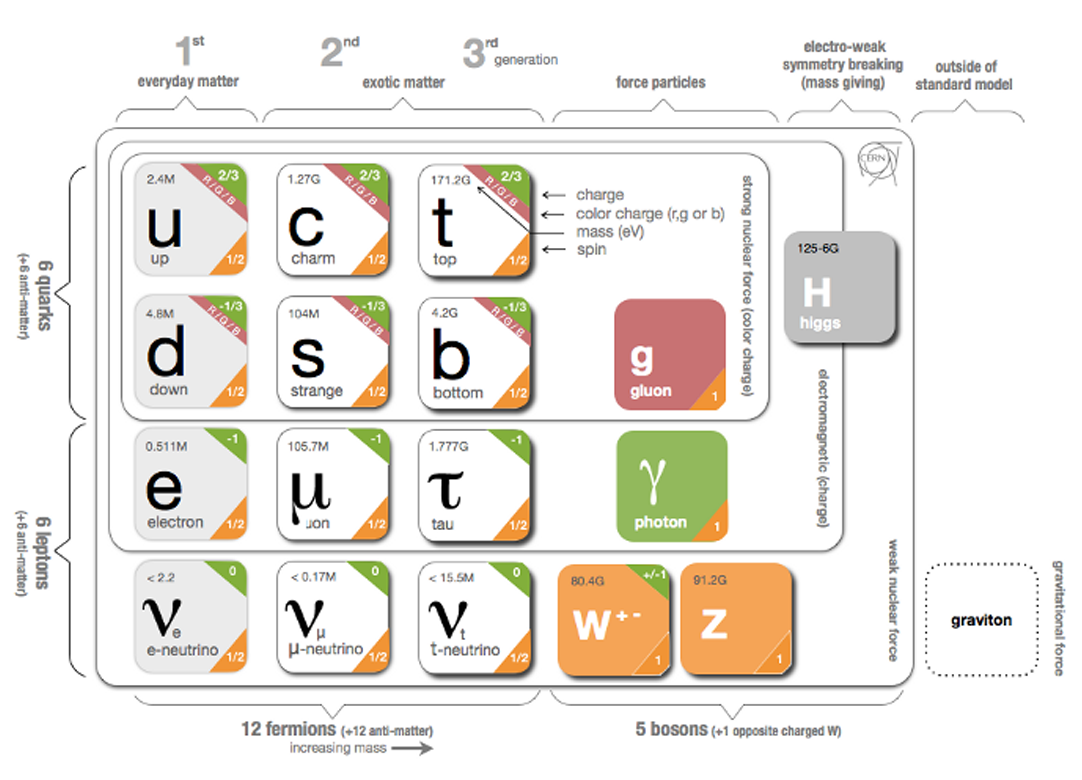
\includegraphics[width=.85\linewidth]{figures/theory/standardmodel.png}
\caption{The Standard Model of particle physics. \cite{Galbraith:2012}}
\label{fig:sm}
\end{figure}
\end{centering}




\subsection{Matter}

The matter described by the \ac{SM} is made up of fermions, spin-$\frac{1}{2}$ particles which can be broken into two groups, quarks and leptons. The leptons all interact weakly, while the quarks additionally interact strongly. 

\subsubsection{Leptons}

Leptons, as seen in the bottom left of \autoref{fig:sm}, come in three generations, each labeled by a flavor: electron, muon, and tau. In the case of the massive leptons, these flavors are mass eigenstates, and the generations are placed in an order based on increasing mass. Thus, the first generation massive lepton, the electron, is stable. Each massive lepton is negatively charged and has a positively charged anti-particle. 

The three neutrinos come in the same flavors as the massive leptons, but these flavor eigenstates do not correspond exactly to mass eigenstates. As a consequence, neutrinos oscillate between flavors as they propagate through space. These oscillations are the only evidence of neutrino mass, which is bound from below by the mass splittings determined from the oscillation. Though it is still uncertain if the masses of the neutrinos follow the same hierarchy as the massive leptons, that expected ordering is slightly preferred over the inverted hierarchy. \cite{Huang:2016} 

Unlike the massive leptons, the neutrinos are uncharged, and it is not yet known whether each neutrino has a separate anti-particle, or if it is its own antiparticle. Because they are uncharged, they can only interact weakly, making them extremely difficult to detect. In the ATLAS detector, neutrinos pass through all layers undetected, and their presence can only be inferred from the non-conservation of momentum that results in the observed particles. As a consequence of their ability to evade detection, neutrinos are the least understood particles of the \ac{SM}. 


\subsubsection{Quarks}


\subsection{Forces}

\subsection{The Higgs Particle}

\subsection{Phenomenology of Proton-Proton Collisions}
\subsubsection{Parton Distribution Functions}

%------------------------------------------------

\subsection{Problems in the Standard Model}
\label{sec:sm_problems}


%------------------------------------------------

\section{Supersymmetry}

\subsection{Supersymmetry Phenomenology}
\subsection{Solutions to Standard Model Problems}
\subsection{Supersymmetry Signatures in $p-p$ Collisions}
\subsubsection{Simplified Models Used in This Analysis}
\label{sec:simplified_models}

\section{Monte Carlo Generators}
\label{sec:MC_gen}